%% Chapter 1
\chapter{Introduction} % Main chapter title
\label{chapterIntroduction} 
%%%%%%%%%%%%%%%%%%%%%%%%%%%%%%%%%%%%%%%%%%%%%%%%%%
%%%%%%%%%%%                                                     %%%%%%%%%%%%%%%%%%%%%%%%%%%
%%%%%%%%%%%           1.1   Consumer RGBD Cameras                   %%%%%%%%%%%%%%%%%%%%
%%%%%%%%%%%                                                     %%%%%%%%%%%%%%%%%%%%%%%%
%%%%%%%%%%%%%%%%%%%%%%%%%%%%%%%%%%%%%%%%%%%%%%%%%%%
\section{RGBD Cameras}
\indent
A Red-Green-Blue-Depth (RGB-D) camera is a sensing system that captures RGB images along with per-pixel depth information. Usually it is simply a combination of a RGB sensor and a depth sensor with an alignment algorithm. Ever since the KinectV1 brought low-cost depth cameras to the consumer market, simple 2D scenes are not able to meet the social demands any more. With the fast development of multimedia technologies, three-dimensional scene display has become a hotspot in the display field. As an extension of classic 2D video, the 3D dynamic display technology can provide a more comprehensive immersive feeling to users than a 2D video. Gesture recognition, 3D modeling, 3D printing, augmented reality, virtual reality, \textit{etc}., a lot of ongoing researches and applications on depth cameras are famous now, cooperated with Human Computer Interaction (HCI) technologies. %
\\\indent%
The PrimeSense's technology had been originally applied to gaming, with user interfaces based on gesture recognition instead of using a controller (also called Natural User Interface, NUI \cite{BraveNUIworld_2011}). It was best known for licensing the hardware design and chip used in Microsoft's first generation of Kinect motion-sensing system for the Xbox 360 in 2010 \cite{PrimeSenseInfo_2013}. The PrimeSense sensor projects an infrared speckle pattern, which will then be captured by an infrared camera in the sensor. A special microchip is employed to compare the captured speckle pattern part-by-part to reference patterns stored in the device, which were captured previously at known depths. The final per-pixel depth will be estimated based on which reference patterns the captured pattern matches best \cite{Krystof12}. Other than the first generation of Kinect camera, Asus Xtion PRO sensor, another consumer NUI application product, has also applied the PrimeSense's technology \cite{AsusXtion_2013}.
\\\indent%
As a competitor \cite{evaluationBetween_2015} of PrimeSense Structured Light technology, time-of-flight technology had been applied into PMD[Vision] CamCube cameras and 3DV's ZCam cameras. Based on known speed of light, Time-of-Flight (ToF) camera resolves distance by measuring the \enquote{time cost} of a special light signal traveling between the camera and target for every single point. The \enquote{time cost} variable that ToF camera measures is the phase shift between the illumination and reflection, which will be translated to distance \cite{TimeOfFlight}. To detect the phase shifts, a light source is pulsed or modulated by a continuous wave, typically a sinusoid or square wave. The ToF camera illumination is typically from a LED or a solid-state laser operating in the near-infrared range invisible to human eyes. Fabrizio \textit{et al}. \cite{depthTechCompare_2011} compared the time-of-flight (PMD[Vision] CamCube) camera and PrimeSense (first generation Kinect) camera in 2011. He showed that the time-of-flight technology is more accurate and claimed that the time-of-flight technology will not only be extended to support colours and higher frame sizes, but also rapidly drop in price. %
% In 2009, 3DV agreed to sell its ZCam assets to Microsoft.
In 2010, it was announced that Microsoft would acquire Canesta for an undisclosed amount \cite{Canesta_2010}. %
And in 2013,  Microsoft released the Xbox One, whose NUI sensor KinectV2 features a wide-angle Canesta ToF camera.
\\\indent
Unlike the PrimeSense's speckle pattern or KinectV2's ToF, Intel RealSense camera utilizes stereo vision \cite{RealSense01_2015}. Its sensor actually has three cameras: two IR cameras (left and right), and one RGB camera. Additionally, RealSense camera also has an IR laser projector to help the stereo vision recognize depth at unstructured surfaces. Compared with KinectV2 camera, RealSense camera is more like a desktop usage to capture faces or even finger gestures, whereas the KinectV2 could do better to capture the full body actions with all joints \cite{RealSense02_2016}. The effective distances of KinectV2 and RealSense hardwares are different. The KnectV2 is optimized to 0.5m ~4.5m, while RealSense are designed for 0.2m~1.2m depends on different devices.

%%%%%%%%%%%%%%%%%%%%%%%%%%%%%%%%%%%%%%%%%%%%%%%%%%
%%%%%%%%%%%                                                                %%%%%%%%%%%%%%%%%
%%%%%%%%%%     1.2  Human Computer Interface                %%%%%%%%%%%%%%%%%%%%
%%%%%%%%%%%                                                                %%%%%%%%%%%%%%%%%%
%%%%%%%%%%%%%%%%%%%%%%%%%%%%%%%%%%%%%%%%%%%%%%%%%%%
\section{Human Computer Interface}
%%
%%
%%
%% gesture recognition
\indent
Gesture recognition is one of the hottest sustained research activities in the area of HCI \cite{NIRGesture14}. It has a wide area of application including human machine interaction, sign language, immersive game technology \textit{etc}. Being a significant part in non-verbal communication, hand gestures are playing vital role in our daily life. Hand Gesture recognition system provides us an innovative, natural, user friendly way of interaction with the computer. By keeping in mind the similarities of human hand shape with four fingers and one thumb, Meenakshi \cite{gestureRecognition12} presents a real time system for hand gesture recognition on the basis of detection of some meaningful shape based features like orientation, center of mass (centroid), status of fingers, thumb in terms of raised or folded fingers of hand and their respective location in image. Since gestures based on hand and finger movements can be robustly understood by computers by using a special 3D IR camera, users are allowed to play games and interact with computer applications in natural and immersive ways that improve the user experience. 
\\\indent
Kam \textit{et al}. \cite{KinectGesture12} developed a real-time gesture-driven human computer interface using the KinectV1 camera and achieved close to 100\% practical recognition rates. After Kam, a Kinect-based calling gesture recognition scenario is proposed by Xinshuang  \textit{et al}. \cite{gestureKinect14} for taking order service of an elderly care robot. Its proposed scenarios are designed mainly for helping non expert users like elderly to call service robot for their service request. In order to facilitate elderly service, natural calling gestures are designed to interact with the robot. Figure~\ref{KinectBasedCallingGesture} shows the evaluation of gesture recognition when sitting on chair. Individual people is segmented out from 3D point cloud acquired by Microsoft Kinect, skeleton is generated for each segment, face detection is applied to identify whether the segment is human or not, and specific natural calling gestures are designed based on skeleton joints. %
\begin{figure}[t]
\centering
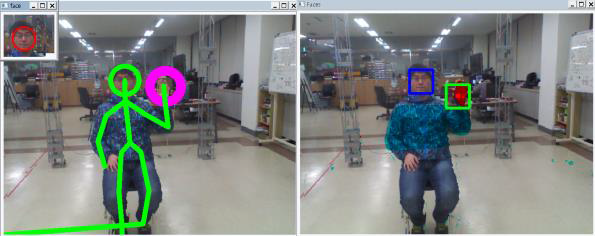
\includegraphics[width=0.65\textwidth]{KinectBasedCallingGesture}
\caption{Calling Gesture Recognition Using Kinect \cite{gestureKinect14}}
\label{KinectBasedCallingGesture}
\end{figure}%
%
\begin{figure}[b]
\centering
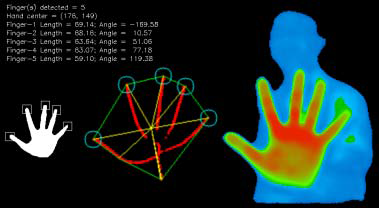
\includegraphics[width=0.75\textwidth]{FingerDetectionUsingDepthData}
\caption{Finger Detection using Depth Data \cite{NIRGesture14}}
\label{FingerDetectionUsingDepthData}
\end{figure}%
Dan \textit{et al}. \cite{NIRGesture14} proposed another smart and real-time depth camera based on a new depth generation principle. A monotonic increasing and decreasing function is used to control the frequency and duty-cycle of the NIR illumination pulses. The adjusted light pulses reflect off of the object of interest and are captured as a series of images. A reconfigurable hardware architecture calculates the depth-map of the visible face of the object in real-time from a number of images. The final depth map is then used for gesture detection, tracking and recognition. Figure~\ref{FingerDetectionUsingDepthData} shows an example extraction of hand skeleton. In 2013, Jaehong \textit{et al}. \cite{InteractiveManipulation_2013} develop and implement a Kinect-based 3D gesture recognition system for interactive
manipulation of 3D objects in educational visualization softwares. 
\\\indent%
%
%%%%
%%%
%%%
%%% SLAM --> accuracy
%%%
%%% indoor perception, SLAM, 
RGB-D cameras own great credits in mobile robotics building dense 3D maps of indoor environments. Such maps have applications in robot navigation, manipulation, semantic mapping, and telepresence. Peter \textit{et al}. \cite{indorMappingRGBD_2014} present a detailed RGB-D mapping system that utilizes a joint optimization algorithm combining visual features and shape-based alignment. Building on best practices in Simultaneous Localization And Mapping (SLAM) and computer graphics makes it possible to build and visualize accurate and extremely rich 3D maps with RGB-D cameras. Visual and depth information are also combined for view-based loop closure detection, followed by pose optimization to achieve globally consistent maps. SLAM is the process of generating a model of the environment around a robot or sensor, while simultaneously estimating the location of the robot or sensor relative to the environment. SLAM has been performed in many ways, which can be categorized generally by their focus on localization or environment mapping \cite{SLAMintro_2015}. SLAM systems focused on localizing the sensor accurately, relative to the immediate environment, make use of sparse sensor data to locate the sensor. Using range sensors such as scanning laser range-finders \cite{laserSLAM_2011}, LiDAR and SONAR \cite{sonarSLAM_2013}, many robot applications use SLAM systems only to compute the distance from the sensor to the environment. SLAM systems focused on mapping use dense sensor output to create a high-fidelity 3D map of the environment, while using those data to also compute relative location of the sensor \cite{KinectFusion_2011, mapSLAM_2013}. Many modern SLAM algorithms combine both approaches, usually by extracting sparse features from the sensor and using these for efficiently computing the location of the sensor. This position is then used to construct a map from dense sensor data. 
\\\indent
With a consumer RGB-D camera providing both color images and dense depth maps at full video frame rate, there appears a novel approach to SLAM that combines the scale information of 3D depth sensing with the strengths of visual features to create dense 3D environment representations, which is called RGB-D SLAM. Felix \textit{et al}. \cite{RGBDSLAM01_2012} gives an open source approach to visual SLAM from RGB-D sensors, which extracts visual keypoints from the color images and uses the depth images to localize them in 3D. %
%
\begin{figure}[t]
\centering
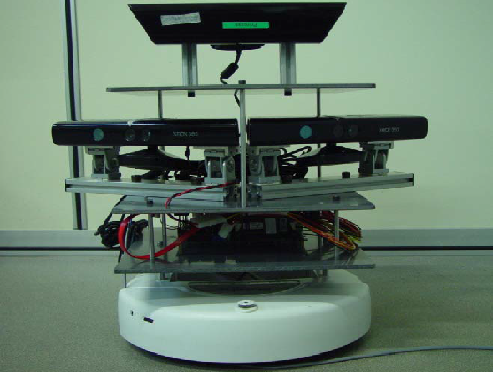
\includegraphics[width=0.5\textwidth]{threeKinect}
\caption{SLAM system with Only RGBD Cameras \cite{RGBDSLAMsystem_2013}}
\label{threeKinect}
\end{figure}%
%
Maohai \textit{et al}. \cite{RGBDSLAMsystem_2013} builds an efficient SLAM system using three RGBD sensors. As shown in Fig.~\ref{threeKinect}, one Kinect looking up toward the ceiling can track the robot's trajectory through visual odometry method, which provide more accurate motion estimation compared to wheel motion measurement without being disturbed under wheel slippage. And the other two contiguous horizontal Kinects can provide wide range scans, which ensure more robust scan matching in the RBPF-SLAM framework. Also using RGB-D sensor for SLAM, Kathia \textit{et al}. \cite{bundleSLAMRGBD_2015} presents a constraint bundle adjustment which allows to easily combine depth and visual data in cost function entirely expressed in pixel. In order to enhance the instantaneity of SLAM for indoor mobile robot, Guanxi \textit{et al}. \cite{indorRGBDSLAM_2015} proposed a RGBD SLAM method based on Kinect camera, which combined Oriented FAST and Rotated BRIEF (ORB) algorithm with Progressive Sample Consensus (PROSAC) algorithm to execute feature extracting and matching. %
%
%
ORB algorithm which has better property than many other feature descriptors was used for extracting feature. At the same time, ICP algorithm was adopted for coarse registration of the point clouds, and PROSAC algorithm which is superior than RANSAC in outlier removal was employed to eliminate incorrect matching. To make the result more accurate, pose-graph optimization was achieved based on General Graph Optimization (g2o) framework. Figure~\ref{3DpointCloudMapOfLab} shows the 3D volumetric map of the lab, which can be directly used to navigate robots.
\\\indent%
%%
%A robot, for example, needs to know its location in the world to navigate between places. This problem is a classical and challenging chicken-and-egg problem because localizing the camera in the world requires the 3D model of the world, and building the 3D model in turn requires the pose of the camera. Therefore, both the camera trajectory and the 3D model need to be estimated at the same time.
\begin{figure}[t]
\centering
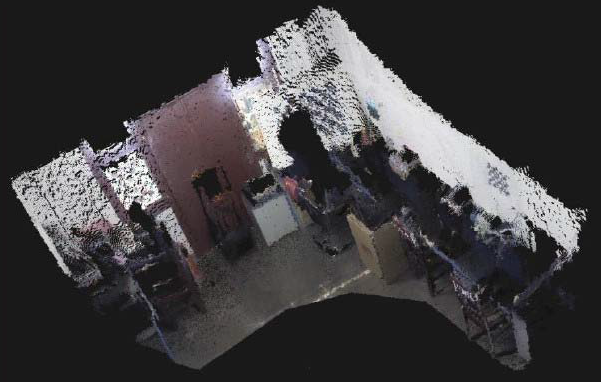
\includegraphics[width=0.7\textwidth]{3DpointCloudMapOfLab}
\caption{3D Map of RGBD-SLAM with ORB and PROSAC \cite{indorRGBDSLAM_2015}}
\label{3DpointCloudMapOfLab}
\end{figure}%
%
RGB-D camera is also famous in application of doing visual odometry on autonomous flight of a micro air vehicle (MAV), helping acquire 3D models of the environment and estimate the camera pose with respect to the environment model. Visual odometry generally has unbounded global drift while estimating local motion. To bound estimation error, it can be integrated with SLAM algorithms, which employ loop closing techniques to detect when a vehicle revisits a previous location. A computationally inexpensive RGBD-SLAM solution tailored to the application on autonomous MAVs is discussed by Sebastian and Andreas \cite{RGBDSLAMmav_2013}, which enables our MAV to fly in an unknown environment and create a map of its surroundings completely autonomously, with all computations running on its onboard computer. Figure~\ref{RGBD_SLAM_MAV} shows the MAC with an RGB-D sensor (the first generation of Kinect) mounted. And Fig.~\ref{mavReconstruction} shows the reconstruction based on the full point clouds, with the estimated trajectory shown in red dots. 
%
\\\indent
%
\begin{figure}[t]
\centering
\subfloat[RGBD UAV]{
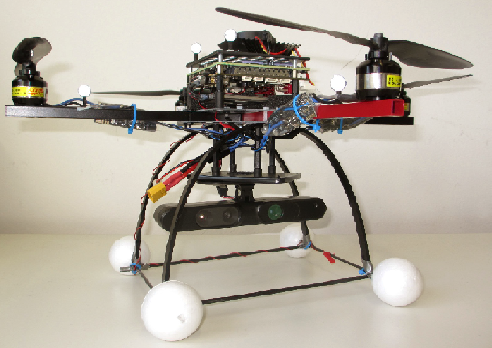
\includegraphics[height=0.4\textwidth , width = 0.5\textwidth]{RGBD_SLAM_MAV}
\label{RGBD_SLAM_MAV}}
\subfloat[Reconstruction and Estimated Trajectory]{
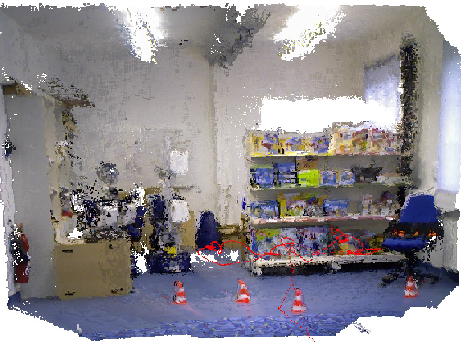
\includegraphics[height=0.4\textwidth , width = 0.5\textwidth]{mavReconstruction}
\label{mavReconstruction}}
%\qquad
\caption{RGBD-SLAM for Autonomous MAVs \cite{RGBDSLAMmav_2013}}
\label{autoRGBD_SLAM_MAV}
\end{figure}%
% Volumetric Reconstruction and Virtual Reality : 3D printing, Kinect fusion
% KinectFusion, 3D printing
RGB-D sensors can be used on a much smaller scale than SLAM to create more detailed, volumetric reconstructions of objects and smaller environments, which opens a new world to the fast 3D printing. 3D printing is an additive technology in which 3D objects are created using layering techniques of different materials, such as plastic, metal, \textit{etc}.  It has been around for decades, but only recently is available and famous among the general public. The first 3D printing technology developed in the 1980's was stereolithography (SLA) \cite{Patent3Dprinting86}. This technique uses an ultraviolet (UV) curable polymer resin and an UV laser to build each layer one by one. Since then other 3D printing technologies have been introduced. Nowadays, some companies like iMaterialise or Shapeways offer 3D printing services where you can simply upload your CAD model on-line, choose a material and in a few weeks your 3D printed object will be delivered to your address. This procedure is quite straight-forward when you got your CAD model. However, 3D shape design tends to be a long and tedious process, with the design of a detailed 3D part usually requiring multiple revisions. Fabricating physical prototypes using low cost 3D fabrication technologies at intermediate stages of the design process is now a common practice, which helps the designer discover errors, and to incrementally refine the design \cite{3DModelingForPrinting15}. Most often, implementing the required changes directly in the computer model, within the 3D modeling software, is more difficult and time consuming than modifying the physical model directly using hand cutting, caving and sculpting tools, power tools, or machine tools. When one of the two models is modified, the changes need to be transferred to the other model, a process we refer to as synchronization. 
\\\indent
KinectFusion, a framework that allows a user to create a detailed 3D reconstruction of an object or a small environment in real-time using Microsoft Kinect sensor, has garnered a lot of attention in the reconstruction and modeling field. It enables a user holding and moving a standard Kinect camera to rapidly create detailed 3D reconstructions of an indoor scene \cite{KinectFusionIzadi_2011}. Not only an entire scene, a specific smaller physical object could also be cleanly segmented from the background model simply by moving the object directly. Figure~\ref{FastDirectObjectSegmentation} shows how the interested object (a teapot) is accurately segmented from the background by physically removed. The sub-figure (A) shows surface normals, and sub-figure (B) is the texture mapped model. %
%
\begin{figure}[t]
\centering
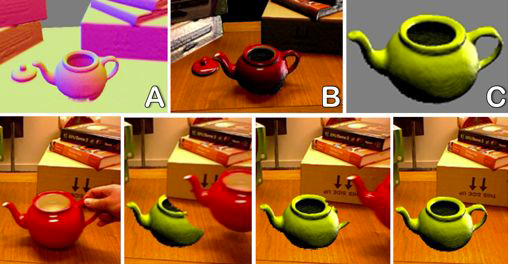
\includegraphics[width=0.7\textwidth]{FastDirectObjectSegmentation}
\caption{Object Segmentation in KinectFusion \cite{KinectFusionIzadi_2011}}
\label{FastDirectObjectSegmentation}
\end{figure}%
%
Nadia \textit{et al}. \cite{3DPrintingFrom3DSensing13} proposed and introduced a from-Sense-to-Print system that can automatically generate ready-to-print 3D CAD models of objects or humans from 3D reconstructions using the low-cost Kinect sensor. Further, Ammar and Gabriel \cite{3DModelingForPrinting15} addresses the problem of synchronizing the computer model to changes made in the physical model by 3D scanning the modified physical model, automatically detecting the changes, and updating the computer model. A new method is proposed that allows the designer to move fluidly from the physical model (for example his 3D printed object, or his carved object) to the computer model. In the proposed process the physical modification applied by the designer to the physical model are detected by 3D scanning the physical model and comparing the scan to the computer model. Then the changes are reflected in the computer model. The designer can apply further changes either to the computer model or to the physical model. Changes made to the computer model can be synchronized to the physical model by 3D printing a new physical model.
%
%
%%%%%%%%%%%%%%%%%%%%%%%%%%%%%%%%%%%%%%%%%%%%%%%%%%
%%%%%%%%%%                                                     %%%%%%%%%%%%%%%%%%%%%%%%%%%
%%%%%%%%%%  1.3   Calibration of RGB-D Cameras         %%%%%%%%%%%%%%%%%%%%%%%%
%%%%%%%%%%                                                     %%%%%%%%%%%%%%%%%%%%%%%%
%%%%%%%%%%%%%%%%%%%%%%%%%%%%%%%%%%%%%%%%%%%%%%%%%%%%%%%
\section{RGB-D Cameras' Calibration and 3D Reconstruction on GPU}
\label{sectionRGBDcameraCalibration}
\indent
 \begin{figure}[b]
%\centering
\subfloat[Front View]{
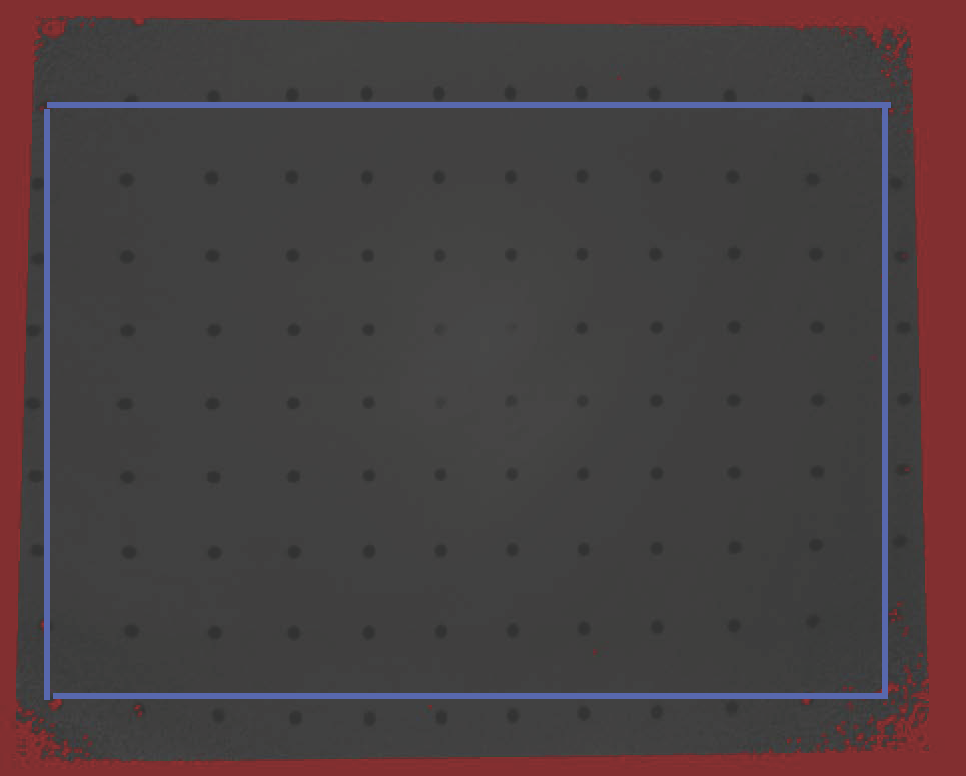
\includegraphics[height=0.42\textwidth]{NIR_by_Depth_front}
\label{NIR_by_Depth_front}}
\subfloat[Side View]{
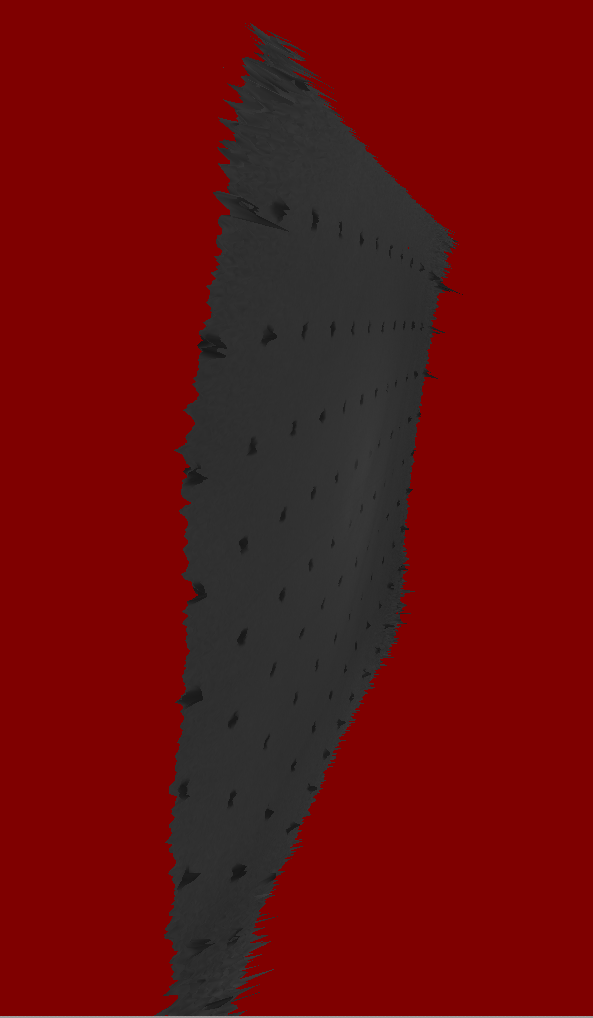
\includegraphics[height=0.42\textwidth , width = 0.4\textwidth]{NIR_by_Depth_LeftSide}
\label{NIR_by_Depth_LeftSide}}
%\qquad
\caption{KinectV2 NearIR 3D Reconstruction in Camera Space}
\label{NearIR}
\end{figure}%
%
As discussed above, applications like RGBD-SLAM and KinectFusion apply 3D reconstruction techniques using an RGBD camera, in which an RGB sensor offers color values and a depth sensor measures objects' distances (\(D\) or \(Z^C\)). RGBD cameras, \text{e.g.} KinectV2, offer the horizontal and vertical field of view (FoV)s of the sensors based on a pinhole camera model, from which a proportional per-pixel beam equation (from \(Z^C\) to \(X^C/Y^C\)) could be derived. It is not hard to do 3D reconstruction in camera space naturally on GPU with the help of the proportional per-pixel beam equations, however, the 3D reconstructed image in that case will be deformed a lot by distortions. Figure~\ref{NearIR} shows the KinectV2 NearIR 3D reconstruction in camera space, when observing a canvas hung on a flat wall printed with uniform grid ground-dots pattern. In the front view, a blue rectangle is drawn based on four corner dot-clusters, which reflects lens distortions (the uniformed distribution of the captured dot-clusters). While in the side view, a blue straight line added on the side of 3D reconstruction, which shows the unflatness of captured \enquote{flat wall}. The deformation in the side view is probably caused by the various resolutions of depth sensor on per-pixel basis, which we will call as \emph{depth distortion} in this thesis. In order to get undistorted 3D images, camera calibration is necessary before a camera being employed.
\\\indent%
%For decades, much work on camera calibration has been done, starting from the photogrammetry community \cite{photogrammetry01_1971, photogrammetry02_1975}, to computer vision (\cite{Tsai1987, treeDcalibration1_1993, Zhengyou04} to cite a few). After the release of the low-cost Microsoft Kinect, a lot of researchers focus their calibrations specially on RGB-D cameras (\textit{e.g.}, Kinect). Jan \textit{et al}. \cite{KinectCali01_2011} analyze Kinect as a 3D measuring device, experimentally investigate depth measurement resolution and error properties and make a quantitative comparison of Kinect accuracy with stereo reconstruction from SLR cameras and a 3D-TOF camera. Using small data sets of Kinect, Carolina \textit{et al}. \cite{KinectCali02_2013} present a new method for calibrating a color-depth camera pair, which prevents the calibration from suffering a drift in scale. Aaron \textit{et al}. \cite{KinectCali03_2015} presented a novel multi-Kinect calibration algorithm that only requires a user to move single spherical object in front of the Kinects observed from multiple viewpoints.
Camera calibration usually use calibration objects, which could be assigned world space coordinates (\(X^W/Y^W/Z^W\)) to help remove distortions. For decades, much work on camera calibration has been done, starting from the photogrammetry community \cite{photogrammetry01_1971, photogrammetry02_1975}, to computer vision (\cite{Tsai1987, treeDcalibration1_1993, Zhengyou04} to cite a few). And the combination of a pinhole-camera matrix with a distortion removal vector (which contains five high-order polynomial parameters) are widely known as important tools in camera calibration. However, there needs to be a lot calculations in the GPU fragment shader based on those parameters from both pinhole-camera matrix and distortion removal vector. And we would like to find a simple method with fewer calculations when generating the 3D coordinates. Similar with the per-pixel \emph{proportional} beam equations in camera space reconstruction on GPU, Kai \cite{Kai10} derived more common \emph{linear} beam equations (from \(X^W\) to \(Y^W/Z^W\)) directly from the pinhole-camera matrix, on the basis of per-pixel. That \emph{linear} beam equations make it possible to show world space 3D reconstruction naturally on GPU, but it did not contains infos about lens distortion correction. 
\\\indent
%
\begin{figure}[t]
\centering
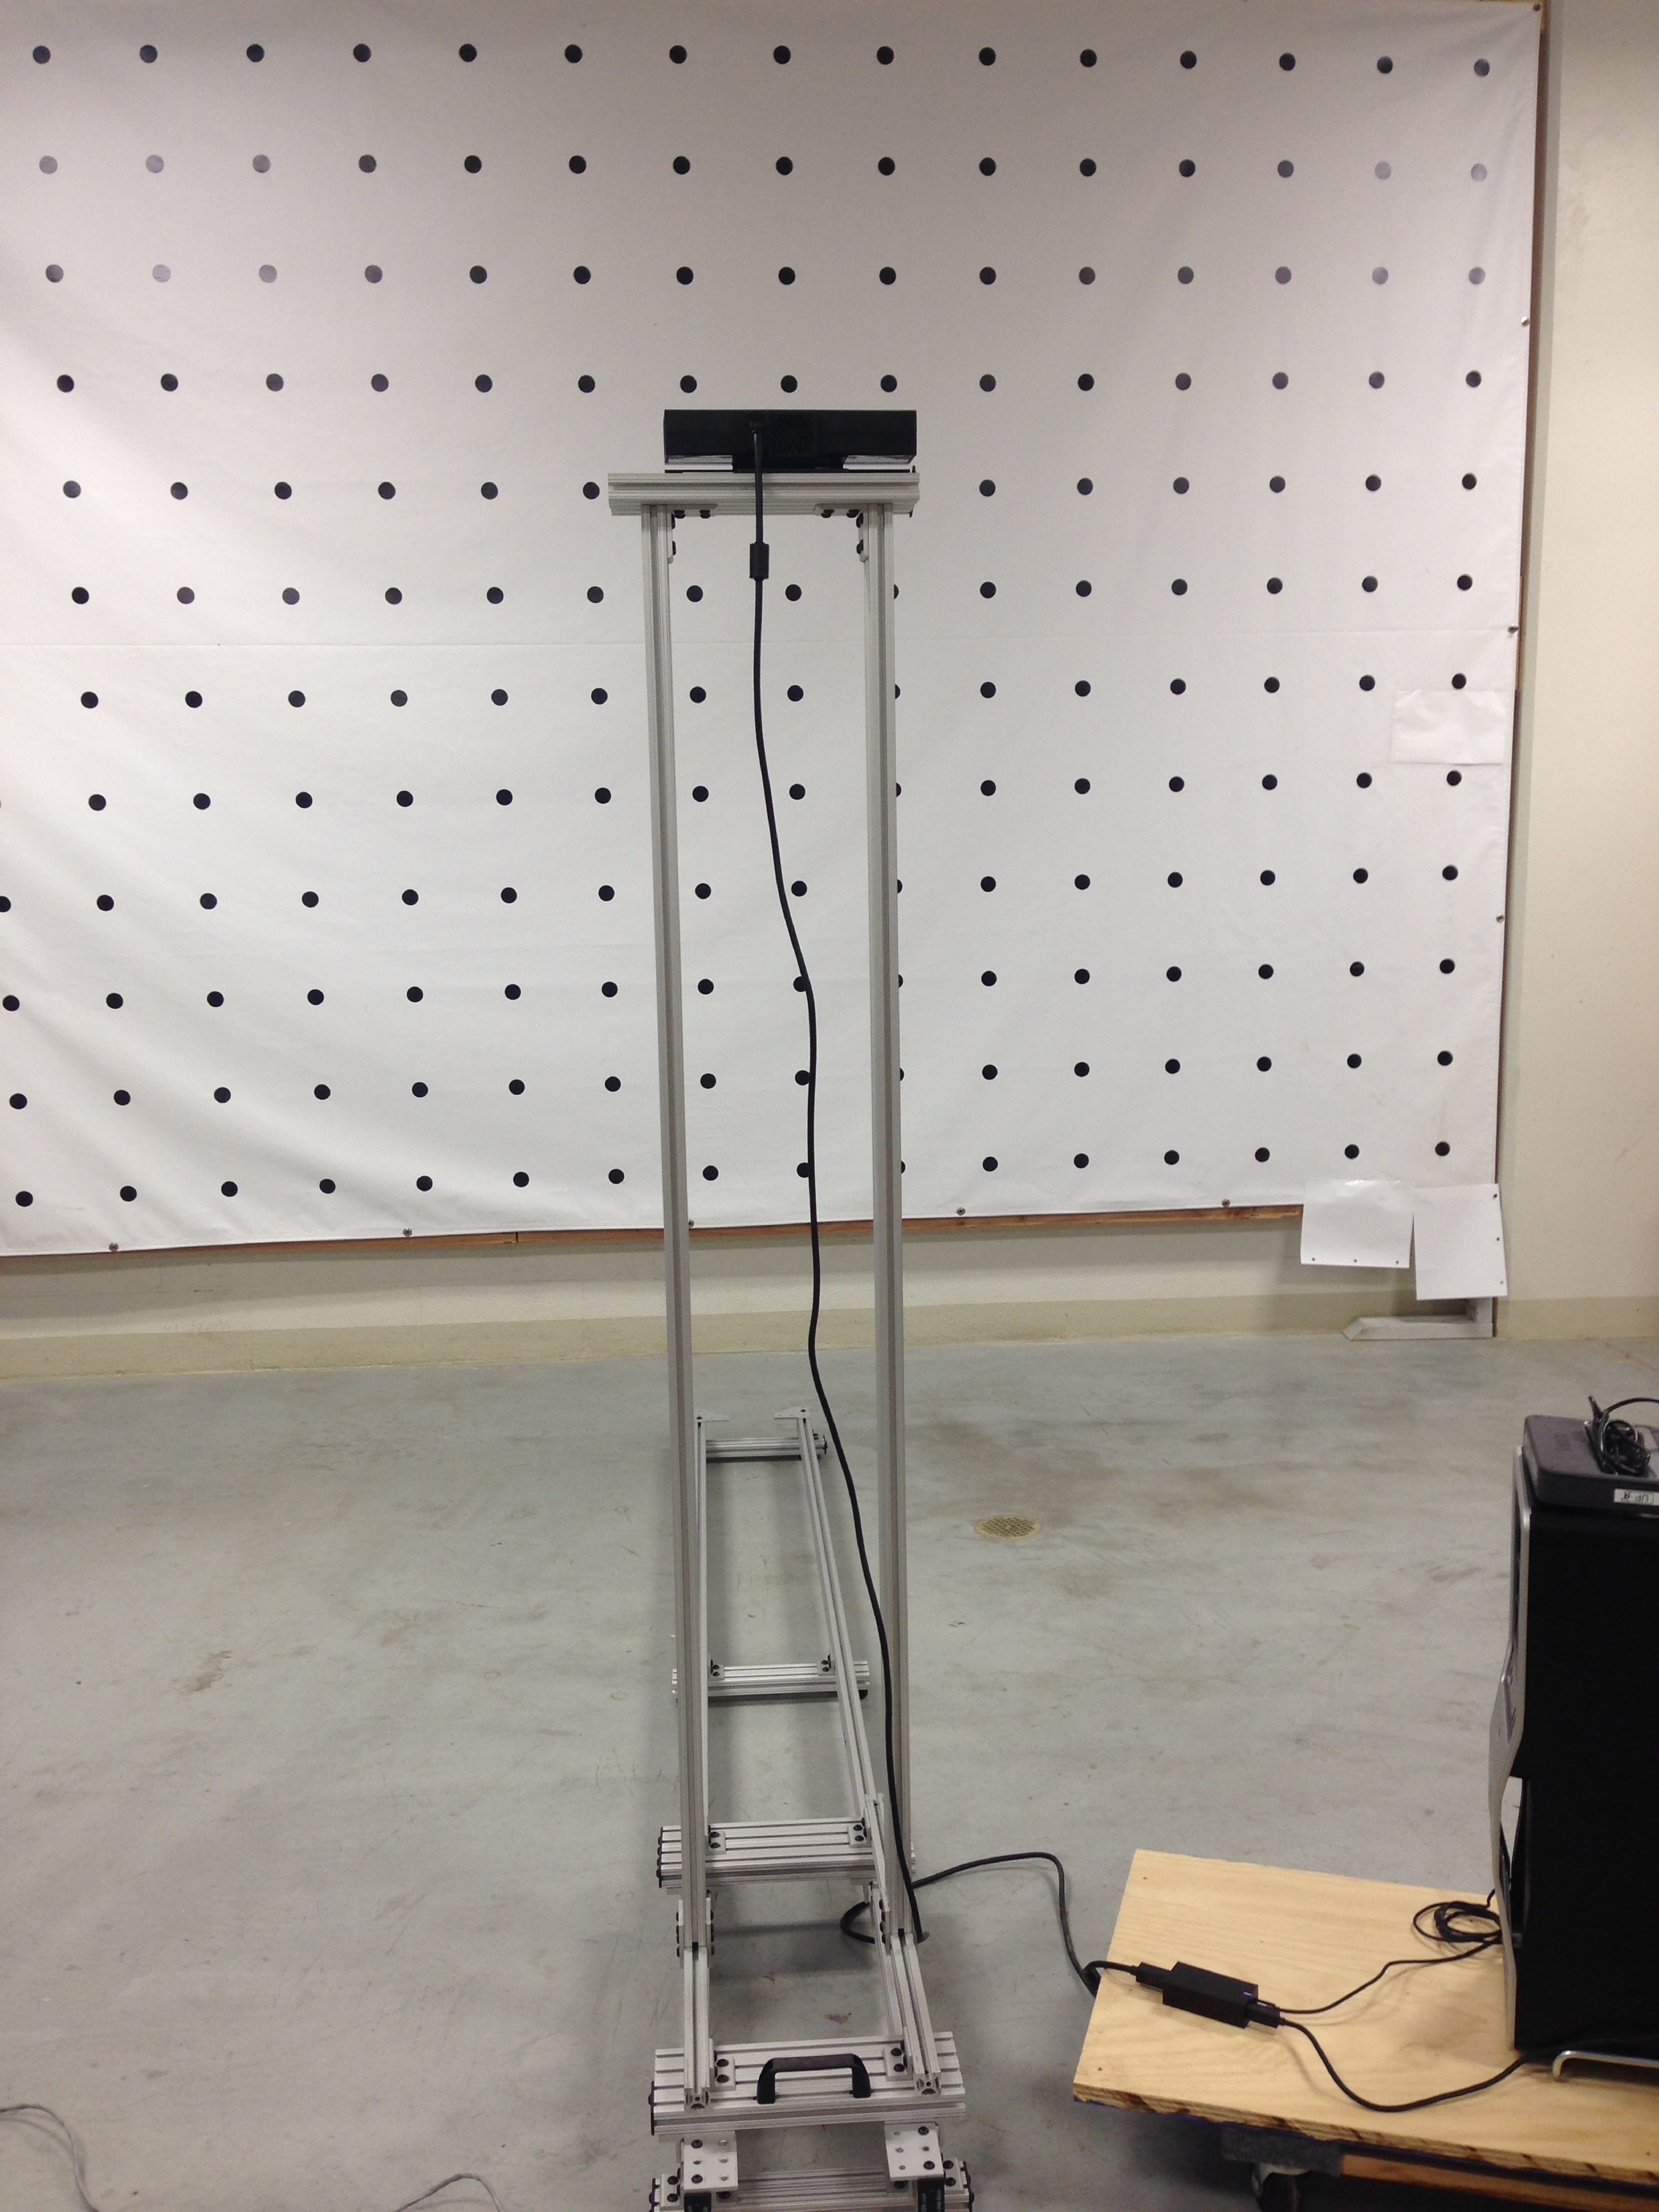
\includegraphics[width=0.55\textwidth]{trackingModuleOnKinectV2CalibrationSystem}
\caption{KinectV2 Calibration System}
\label{trackingModuleOnKinectV2CalibrationSystem}
\end{figure}%
Our goal is to draw undistorted 3D reconstruction on GPU with the fewest calculations. Inspired by Kai, we will build up a rail calibration system to support the per-pixel \(D\) to \(Z^W\) mapping, such that Kai's per-pixel \(X^W\) to \(Y^W/Z^W\) linear mappings could be applied during the 3D reconstruction on GPU. We will call this new method \textit{per-pixel calibration}. As shown in Fig.~\ref{trackingModuleOnKinectV2CalibrationSystem}, the camera observing the uniform grid dots pattern is mounted on a rail, which is perpendicular to pattern on the wall. A laser distance measurer will be used to supply accurate per-frame \(Z^W\), so that the per-pixel \(D\) to \(Z^W\) mapping could handle \emph{depth distortion}. As long as the undistorted dense \(X^W/Y^W\) could be acquired, we will be able determine the parameters of per-pixel \emph{linear} beam equations.
\\\indent
Undistorted world space coordinates \(X^W/Y^W/Z^W\) with \(D\) together will be collected and saved onto local drives, during which lens distortions will be removed. Instead of using the combination of pinhole-camera matrix and distortion removal vector, we will determine a best-fit two--dimensional high-order polynomial mapping that can directly map from \(Row\) and \(Column\) in image space to \(X^W\) and \(Y^W\), and the high-order polynomial mapping will handle the lens distortions. After the data collection, we will determine a best-fit mapping model between per-pixel \(D\) and \(Z^W\), and then process the collected data, and finally generate per-pixel mapping parameters, which can make up a look-up table that will help draw undistorted 3D reconstruction on GPU in real-time.
\\\indent
In Chapter~\ref{chapterTraditionalCalibration}, a pinhole-camera-model based calibration method is discussed in detail, including the lens distortions analysis and its removal. Chapter~\ref{chapterDataBasedCalibration} will introduce how to draw the camera space 3D reconstruction on GPU, introduce a rail calibration system's set-up, and then talk about the proposed per-pixel calibration method and simple 3D reconstruction on GPU in detail. Chapter~\ref{chapterCaliResultsReconstruction} will explain how the two polynomial mapping models in the proposed calibration method are determined, and then show the calibrated results about how well the lens distortions and \emph{depth distortion} are corrected. Chapter~\ref{chapterConclusionAndFutureWork} will conclude this thesis and talk about the future work of RGB-D cameras calibration.

%
%%%%%%%%%%%%%%%%%%%%%%%%%%%%%%%%%%%%%%%%%%%%%%%%%%%%%%%
%%%%%%%%%%                                                     %%%%%%%%%%%%%%%%%%%%%%%%%%%
%%%%%%%%%%  1.4     Summation                         %%%%%%%%%%%%%%%%%%%%%%%%
%%%%%%%%%%                                                     %%%%%%%%%%%%%%%%%%%%%%%%
%%%%%%%%%%%%%%%%%%%%%%%%%%%%%%%%%%%%%%%%%%%%%%%%%%%%%%%
%\section{Summation}
%\label{sectionLastSecInCh1}
%\indent
%A RGB-D camera is a sensing system that capture RGB images along with per-pixel depth information. It opens a new epoch for 3D markets. Ever since the Microsoft brought the low-cost depth camera Kinect into consumer market, RGB-D cameras are famous in a broad research areas of HCI, \textit{e.g.} gesture recognition, SLAM, UAV, KinectFusion, Reconstruction and Virtual Reality, \textit{etc}. Accompanied by its popularity, an accurate camera calibration gets more significance as a preprocessing of RGB-D camera applications in computer vision. Camera calibration aims to solve two types of distortions, perspective distortion and optical distortion, both of which result in some kind of deformation of images.
%\\\indent
%Perspective distortion comes along with the light ray's projection from three dimensional space to a two dimensional image. It appears as linear deformation (extension or compression) in texture, that straight lines of an object still appearing straight, and is caused by the position of the camera relative to the subject. If a subject is too close to the camera, it can appear disproportionately large or distorted when compared to the objects in the background. A pinhole camera model is usually utilized to simulate and explain the light ray's projection from 3D objects to 2D images. It contains the point mapping relationships going from the world domain, through the camera domain, and finally to the image domain; based on which the perspective distortion problem could be solved mathematically.
%\\\indent
%Optical distortion is caused by the optical design of lenses, and is therefore often called \enquote{lens distortion}. Unlike the linear perspective distortion, it physically bends straight lines and makes them appear curvy in images. Imperfect lens shape causes light rays bending more near the edges of a lens than they do at its optical center, which is called \enquote{radial distortion}. Usually for the low-cost consumer camera with wide-angle lenses, where the field of view of the lens is much wider than the size of the image sensor, the deformed image appears like a barrel, so that this radial distortion at this situation is also called a \enquote{Barrel Distortion}. Other than the radial direction, there is also tangential distortion that causes image deformation, which occurs when the lens and the image plane (the sensor) are not parallelly assembled. The lens distortions are usually dominated by radial distortion, and commonly solved by a high order polynomial non-linear model after the correction of perspective distortion.
%\\\indent



%
% However, the traditional camera calibration methods are not ideal on accuracy and efficiency. They do not cover all pixels of a sensor, and did not consider the problem of \enquote{Depth Distortion} either. Besides, those methods need the distortion removal to be a second step after raw 3D reconstruction (from a pinhole camera matrix), which is not an efficient way displaying the 3D reconstruction in real-time.
%
%
%RGB-D cameras have both of lens distortions and depth distortion problems. Distortions correction is wildly discussed in image processing area, however, the traditional camera calibration methods are not ideal on accuracy and efficiency. They separated the lens distortion removal from the 3D reconstruction (based on pinhole camera model), which depresses the efficiency of image processing. Moreover, they neither cover all pixels of a sensor when training the distortion model, nor include the depth distortion correction (assuming that the depth values have exact same resolution among every single pixel).%
%
%
%
%
%
%
%








%
% In this section, we will introduce how to generate the camera space 3D coordinates without calibration, and draw a camera space 3D reconstruction on GPU using a KinectV2 camera.
%
%Camera calibration is a necessary step in 3D computer vision in order to extract metric information from 2D images. The calibration of a RGB-D camera aims to be able to generate the world coordinates (\(X^W, Y^W, Z^W\)) with corresponding \(RGB\) values for every single pixel, given the depth steams and RGB streams retrieved from the camera. During the camera calibration, the removal of lens distortions must be involved in order to get the undistorted 3D reconstruction, especially for consumer cameras that utilize a low-cost lens. Imperfect lens shape causes light rays bending more near the edges of a lens than they do at its optical center. The smaller the lens, the greater the distortion. With a wide-angle lens where the field of view of the lens is much wider than the size of the image sensor, barrel distortions will commonly happen. For example, Fig.~\ref{NIR_by_Depth_front} shows KinectV2's raw (without distortion removal) NearIR 3D image observing a flat wall, on which a canvas printed with uniform grid dots pattern is hung. A blue rectangle is dropped onto the image, which helps show the \enquote{barrel-shape} deformation of the uniform grid pattern.
%\\\indent
%For decades, much work on camera calibration has been done, starting from the photogrammetry community \cite{photogrammetry01_1971, photogrammetry02_1975}, to computer vision (\cite{Tsai1987, treeDcalibration1_1993, Zhengyou04} to cite a few). After the release of the low-cost Microsoft Kinect, a lot of researchers focus their calibrations specially on RGB-D cameras (\textit{e.g.}, Kinect). Jan \textit{et al}. \cite{KinectCali01_2011} analyze Kinect as a 3D measuring device, experimentally investigate depth measurement resolution and error properties and make a quantitative comparison of Kinect accuracy with stereo reconstruction from SLR cameras and a 3D-TOF camera. Using small data sets of Kinect, Carolina \textit{et al}. \cite{KinectCali02_2013} present a new method for calibrating a color-depth camera pair, which prevents the calibration from suffering a drift in scale. Aaron \textit{et al}. \cite{KinectCali03_2015} presented a novel multi-Kinect calibration algorithm that only requires a user to move single spherical object in front of the Kinects observed from multiple viewpoints.
%\\\indent
%%
% \begin{figure}[b]
%%\centering
%\subfloat[Front View][Front View]{
%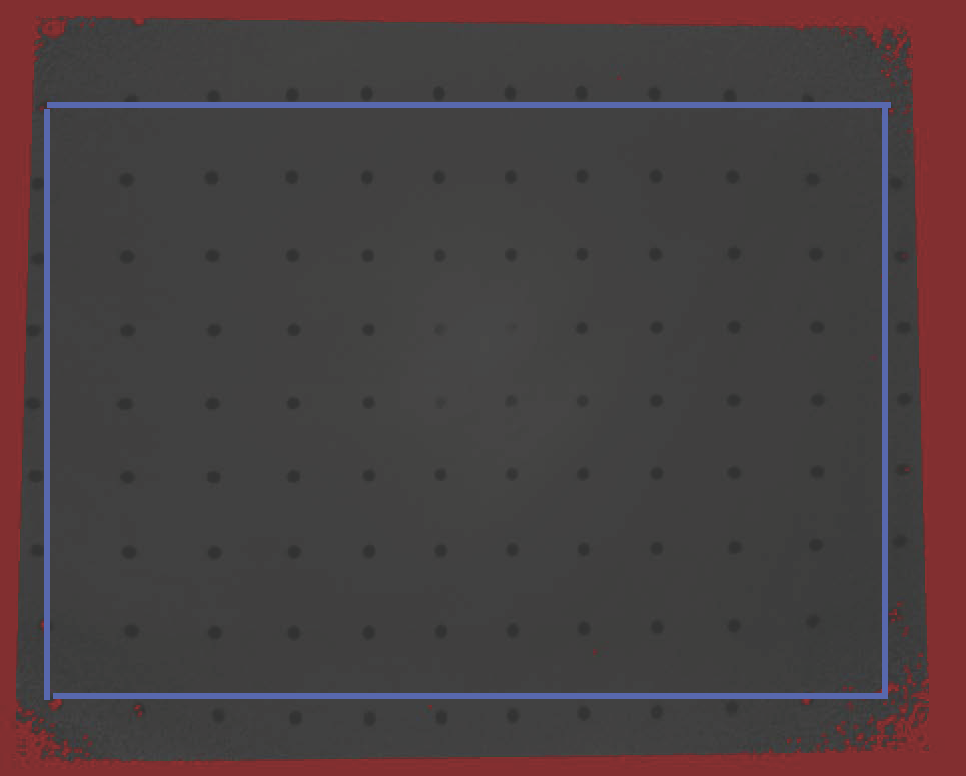
\includegraphics[height=0.42\textwidth]{NIR_by_Depth_front}
%\label{NIR_by_Depth_front}}
%\subfloat[Left View][Left View]{
%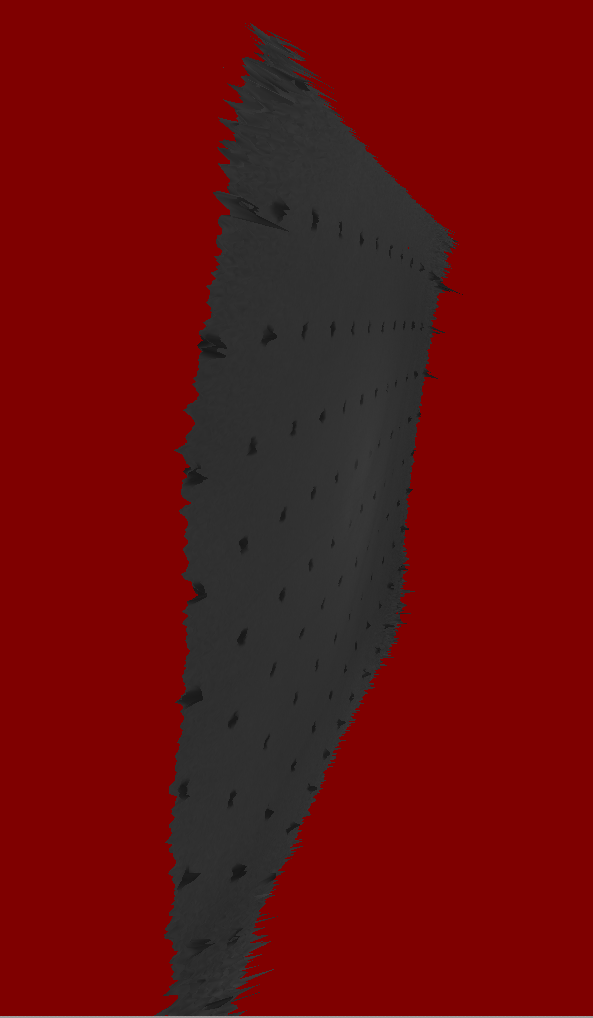
\includegraphics[height=0.42\textwidth , width = 0.4\textwidth]{NIR_by_Depth_LeftSide}
%\label{NIR_by_Depth_LeftSide}}
%%\qquad
%\caption{Raw Distorted KinectV2 NearIR 3D Reconstruction}
%\label{NearIR}
%\end{figure}%
%%
%However, those camera calibration methods, using limited number of points to train the non-linear distortion-removal model, are not able to cover all pixels of a sensor. Besides, with one pinhole camera model (3-by-4 transformation matrix) for raw (deformed) 3D reconstruction and another model to remove lens distortion, the final 3D reconstruction cannot be displayed efficiently in real-time. What's worse, those calibration methods are assuming that the depth sensor offers perfectly same precision depth value for all pixels. Whereas in practical depth sensors always have some defects in getting same depth accuracy for all of their pixels, which we will call as \enquote{Depth Distortion}. Kourosh and Sander \cite{KinectAccuracy_2012} provide an analysis of the accuracy and resolution of Kinect's depth data. They show that the random error of depth measurement increases with increasing distance to the sensor, and ranges from a few millimeters up to about 4 cm at the maximum range of the sensor. Figure~\ref{NIR_by_Depth_LeftSide} shows the side view of KinectV2's raw 3D NearIR image observing the wall, and the blue straight line is added on the left side of the 3D reconstruction. We can tell that most pixels on the left side border are apparently not sitting on a straight line.%
%\\\indent
%%
%\begin{figure}[t]
%\centering
%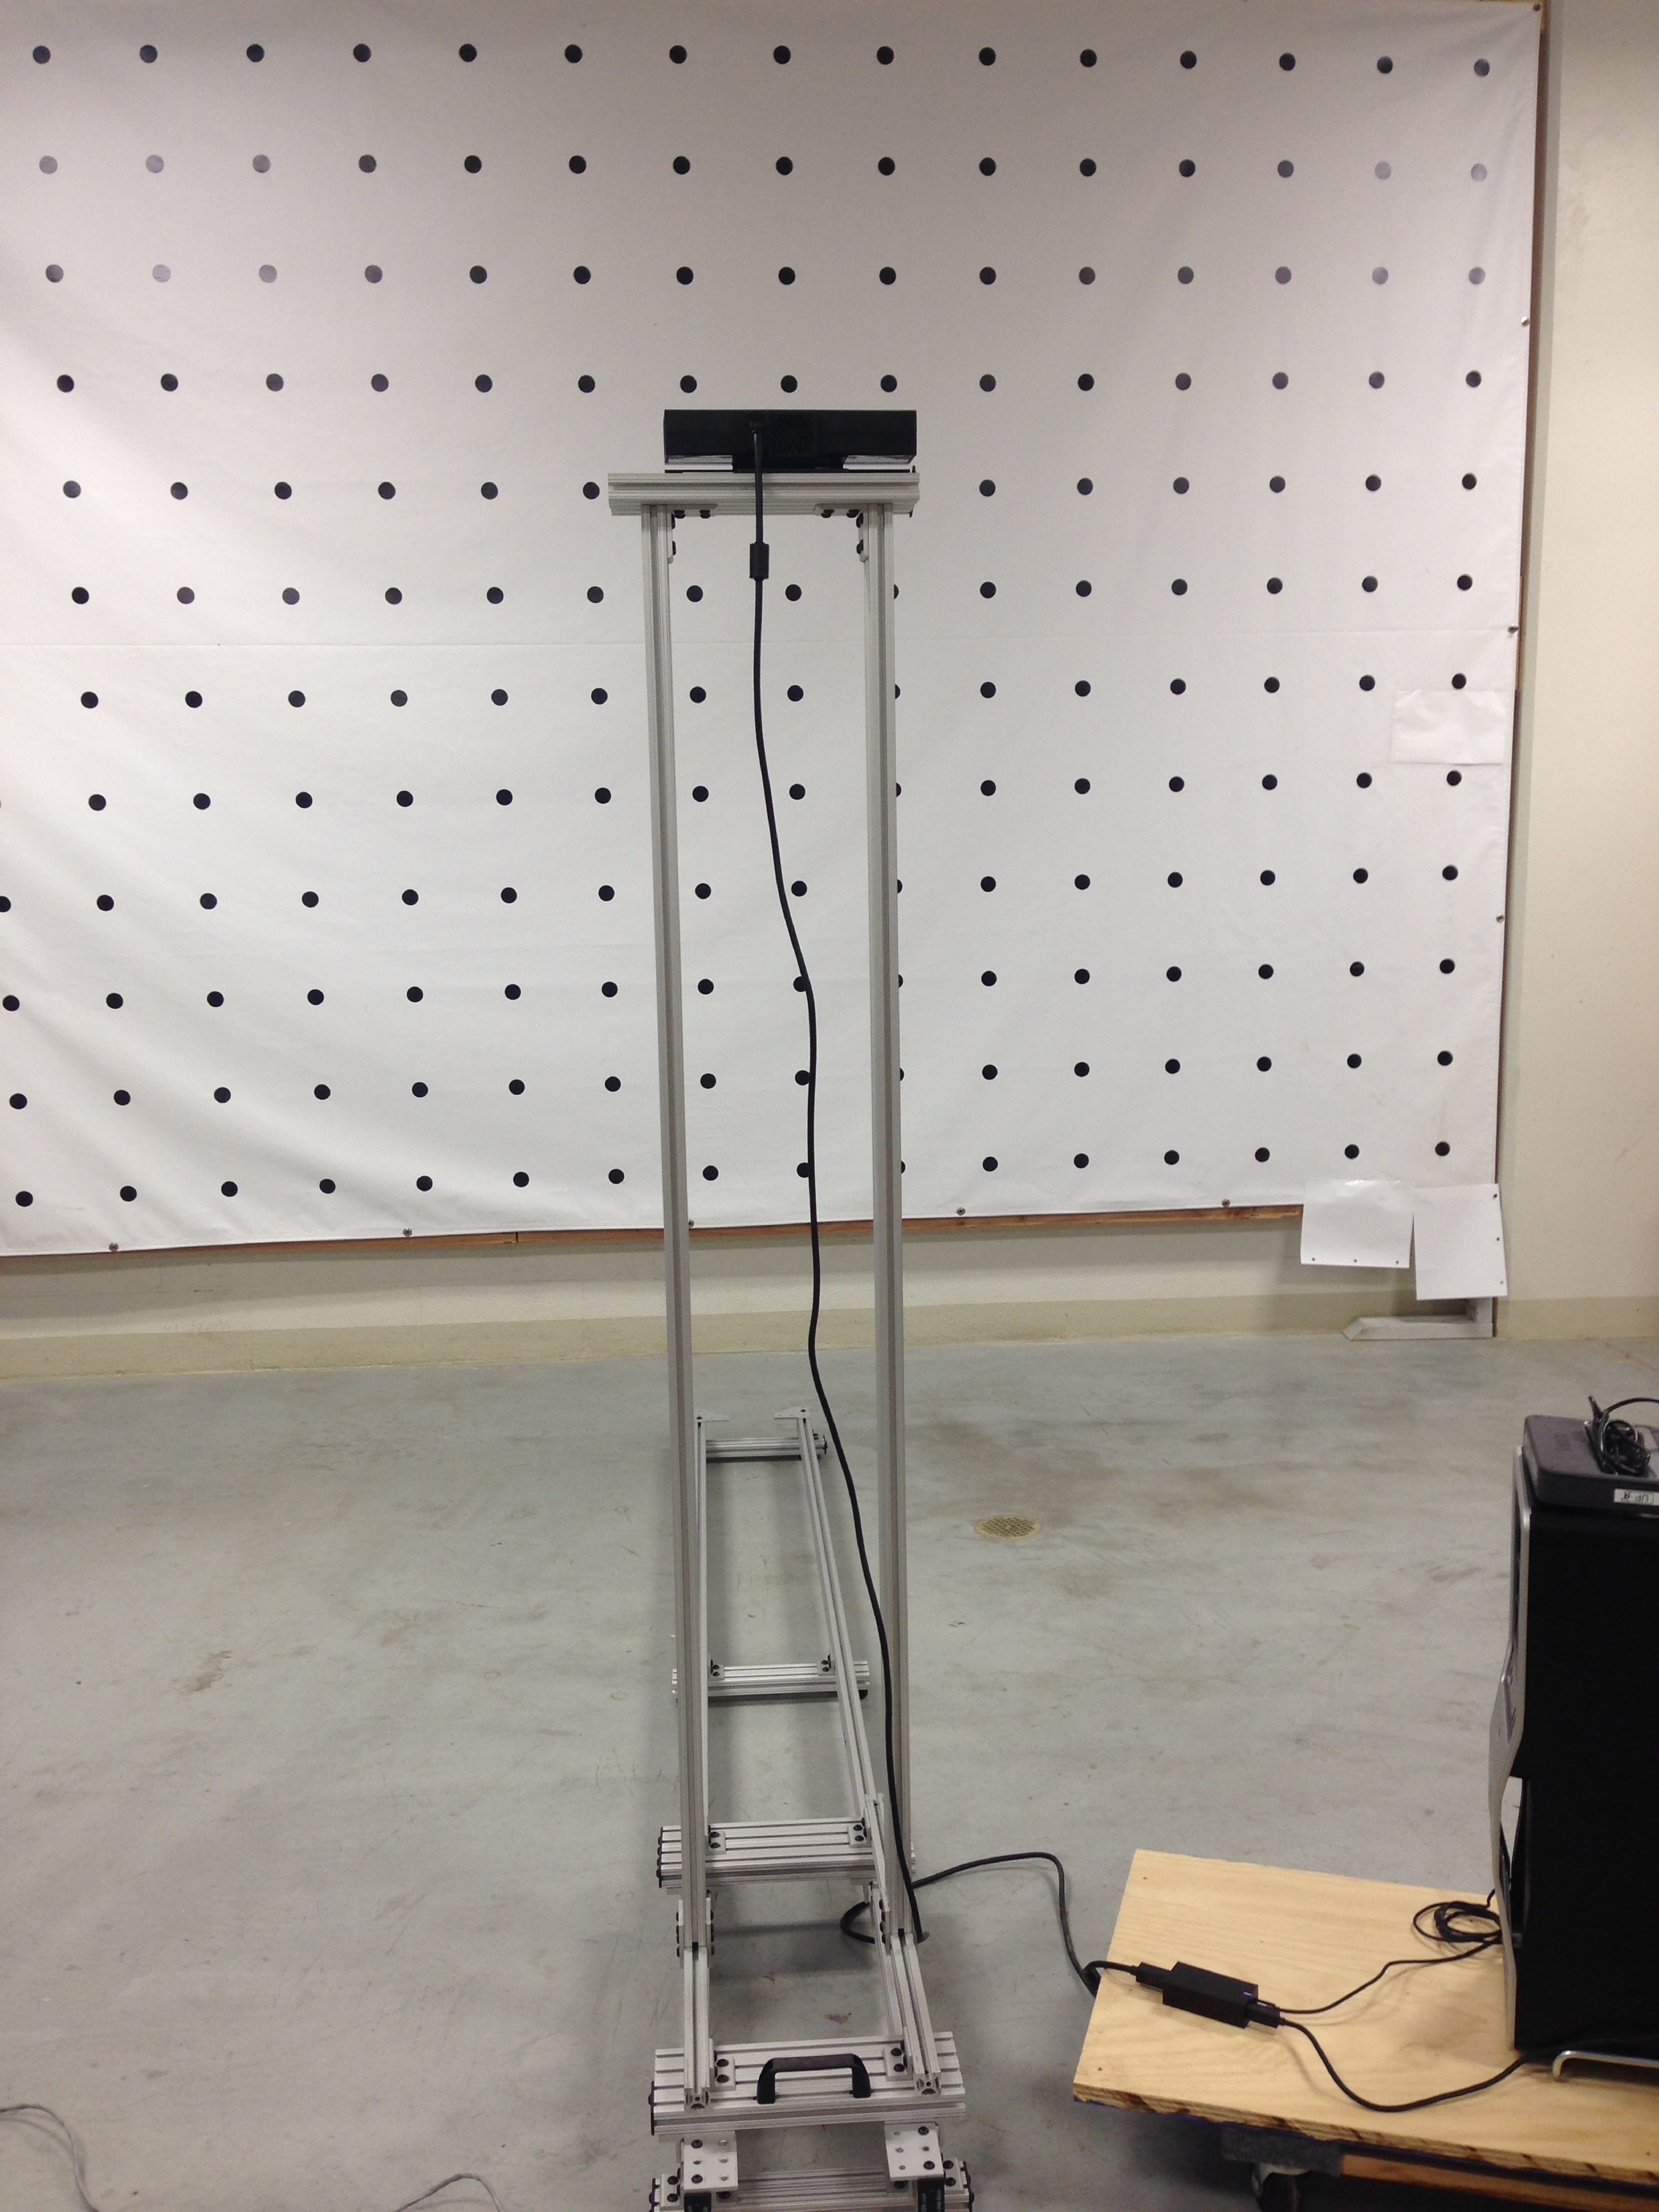
\includegraphics[width=0.55\textwidth]{trackingModuleOnKinectV2CalibrationSystem}
%\caption{KinectV2 Calibration System}
%\label{trackingModuleOnKinectV2CalibrationSystem}
%\end{figure}%
%%
%In order to get enough calibrating points that can cover all pixels of the sensor, as well as solving the \enquote{Depth Distortion}, a moving plane with camera on rail calibration system is introduced in this thesis. As shown in figure \ref{trackingModuleOnKinectV2CalibrationSystem}, the rail is perpendicular to the uniform round dots pattern, along with the \(Z^{w}\) axis. A RGB-D camera KinectV2 is mounted on the top of the slider, whose moving along the rail generates same effect as a moving pattern plane. This calibration system makes it possible to do per-pixel \enquote{Depth Distortion} calibration.%
%%
%%
%%%%%%%%%%%%%%%%%%%%%%%%%%%%%%%%%%%%%%%%%%%%%%%%%%%%%%%%
%%%%%%%%%%%                                                     %%%%%%%%%%%%%%%%%%%%%%%%%%%
%%%%%%%%%%%  1.4     Summation                         %%%%%%%%%%%%%%%%%%%%%%%%
%%%%%%%%%%%                                                     %%%%%%%%%%%%%%%%%%%%%%%%
%%%%%%%%%%%%%%%%%%%%%%%%%%%%%%%%%%%%%%%%%%%%%%%%%%%%%%%%
%\section{Summation}
%\label{sectionLastSecInCh1}
%\indent
%A RGB-D camera is a sensing system that capture RGB images along with per-pixel depth information. It opens a new epoch for 3D markets. Ever since the Microsoft brought the low-cost depth camera Kinect into consumer market, RGB-D cameras are famous in a broad research areas of HCI, \textit{e.g.} gesture recognition, SLAM, UAV, KinectFusion, Reconstruction and Virtual Reality, \textit{etc}. Accompanied by its popularity, an accurate camera calibration gets more significance as a preprocessing of RGB-D camera applications in computer vision. Camera calibration aims to solve two types of distortions, perspective distortion and optical distortion, both of which result in some kind of deformation of images.
%\\\indent
%Perspective distortion comes along with the light ray's projection from three dimensional space to a two dimensional image. It appears as linear deformation (extension or compression) in texture, that straight lines of an object still appearing straight, and is caused by the position of the camera relative to the subject. If a subject is too close to the camera, it can appear disproportionately large or distorted when compared to the objects in the background. A pinhole camera model is usually utilized to simulate and explain the light ray's projection from 3D objects to 2D images. It contains the point mapping relationships going from the world domain, through the camera domain, and finally to the image domain; based on which the perspective distortion problem could be solved mathematically.
%\\\indent
%Optical distortion is caused by the optical design of lenses, and is therefore often called \enquote{lens distortion}. Unlike the linear perspective distortion, it physically bends straight lines and makes them appear curvy in images. Imperfect lens shape causes light rays bending more near the edges of a lens than they do at its optical center, which is called \enquote{radial distortion}. The smaller the lens, the greater the distortion. Usually for the low-cost consumer camera with wide-angle lenses, where the field of view of the lens is much wider than the size of the image sensor, the deformed image appears like a barrel, so that this radial distortion at this situation is also called a \enquote{Barrel Distortion}. Other than the radial direction, there is also tangential distortion that causes image deformation, which occurs when the lens and the image plane (the sensor) are not parallelly assembled. The lens distortions are usually dominated by radial distortion, and commonly solved by a high order polynomial non-linear model after the correction of perspective distortion.
%\\\indent
%
%
%
%
% However, the traditional camera calibration methods are not ideal on accuracy and efficiency. They do not cover all pixels of a sensor, and did not consider the problem of \enquote{Depth Distortion} either. Besides, those methods need the distortion removal to be a second step after raw 3D reconstruction (from a pinhole camera matrix), which is not an efficient way displaying the 3D reconstruction in real-time.
%
%
%RGB-D cameras have both of lens distortions and depth distortion problems. Distortions correction is wildly discussed in image processing area, however, the traditional camera calibration methods are not ideal on accuracy and efficiency. They separated the lens distortion removal from the 3D reconstruction (based on pinhole camera model), which depresses the efficiency of image processing. Moreover, they neither cover all pixels of a sensor when training the distortion model, nor include the depth distortion correction (assuming that the depth values have exact same resolution among every single pixel).%
%\\\indent
%In this thesis, a novel per-pixel calibration method with look-up table based 3D reconstruction in real-time is introduced, using a rail calibration system shown in Fig.~\ref{trackingModuleOnKinectV2CalibrationSystem}. Instead of using a pinhole camera model, which in practical is not ideally accurate, our new proposed calibration method is based on real data. Not only \(X^W\)/\(Y^W\) values are calibrated directly through one step transformation, but \(Z^w\) is also guaranteed accurate by importing externally measured data. Both of the lens distortions and \enquote{depth distortion} could be solved with the help of the rail system.
%\\\indent
%In Chapter 2, a pinhole-camera-model based calibration method is discussed in detail, including the lens distortions removal as the second step. The proposed data-based calibration method is well explained in Chapter 3, where two polynomial models will be introduced. One lens-distortions removal model helps map directly from image plane \(row\) and \(column\) to \(X^{W}\) and \(Y^{W}\) separately, during calibration data collection. And another \enquote{depth distortion} removal model helps map per-pixel depth (\(D\)) to \(Z^W\) when generating look-up table for per-pixel beam equation. \(Z^{w}\) values will be totally supported from external (a laser distance measurer). The calibration results and real-time 3D reconstruction will be discussed in Chapter 4. Finally, a \(row\) by \(column\) by 6, three dimensional look-up table will be generated for real-time 3D reconstruction. Chapter 5 will talk the future work of RGB-D cameras calibration.
%%
%%
%%
%%
%%
%%
%%
%






































































%Noises among depth data vary randomly, camera by camera and pixel by pixel; which means a rough point-cloud plane full of bumps and hollows will be reconstructed even though the camera is observing a wall. 




%
%\begin{table}[ht]
%\begin{center}
%\caption{ 3D profile acquisition Taxonomy}
%\label{3DImagingTaxonomy}
%\hspace*{-1cm}
%\begin{tabular}{ |>{\small}l|>{\small}l|>{\small}l|>{\small}l| }
%\hline
%\multicolumn{4}{|c|}{3D Shape Extraction} \\
%\hline
%\multicolumn{2}{|c|}{Passive}  & \multicolumn{2}{c|}{Active}\\
%\hline
%Single Vantage Point & Multiple Vantage Points & Single Vantage Point & Multiple Vantage Points\\
%\hline
%\multirow{5}{*}{
%\makecell[l]{
%\textbullet \, Shape from Texture\\ 
%\textbullet \, Shape from Occlusion\\
%\textbullet \, Time to Contact\\
%\textbullet \, Shape from Defocus\\
%\textbullet \, Shape from Contour}
%} 
%&
%\multirow{5}{*}{\makecell[l]{
%\textbullet \, Passive Stereo\\ 
%\textbullet \, Structure from Motion\\
%\textbullet \, Shape from Silhouettes}
%}
%&
%\multirow{5}{*}{\makecell[l]{
%\textbullet \, Time of Flight\\ 
%\textbullet \, Shape from Shading}
%} 
%&
%\multirow{5}{*}{\makecell[l]{
%\textbullet \, Structured Light\\ 
%\textbullet \, Active Stereo\\
%\textbullet \, Photometric Stereo}
%} \\ & & &
%\\ & & &	\\ & & &	\\ & & &\\
%\hline
%
%\end{tabular}
%\end{center}
%\end{table}





%
%%%%%%%%%%%%%%%%%%%%%%%%%%%%%%%%%%%%%%%%%%%%%%%%%%%
%%%%%%%%%%%                                                     %%%%%%%%%%%%%%%%%%%%%%%%%%%
%%%%%%%%%%%  1.3   Calibration of RGB-D Cameras         %%%%%%%%%%%%%%%%%%%%%%%%
%%%%%%%%%%%                                                     %%%%%%%%%%%%%%%%%%%%%%%%
%%%%%%%%%%%%%%%%%%%%%%%%%%%%%%%%%%%%%%%%%%%%%%%%%%%%%%%%
%\section{Calibration of RGB-D Cameras}
%\label{sectionRGBDcameraCalibration}
%\indent
%Camera calibration is a necessary step in 3D computer vision in order to extract metric information from 2D images. The calibration of a RGB-D camera aims to be able to generate the world coordinates (\(X^W, Y^W, Z^W\)) with corresponding \(RGB\) values for every single pixel, given the depth steams and RGB streams retrieved from the camera. During the camera calibration, the removal of lens distortions must be involved in order to get the undistorted 3D reconstruction, especially for consumer cameras that utilize a low-cost lens. Imperfect lens shape causes light rays bending more near the edges of a lens than they do at its optical center. The smaller the lens, the greater the distortion. With a wide-angle lens where the field of view of the lens is much wider than the size of the image sensor, barrel distortions will commonly happen. For example, Fig.~\ref{NIR_by_Depth_front} shows KinectV2's raw (without distortion removal) NearIR 3D image observing a flat wall, on which a canvas printed with uniform grid dots pattern is hung. A blue rectangle is dropped onto the image, which helps show the \enquote{barrel-shape} deformation of the uniform grid pattern.
%\\\indent
%For decades, much work on camera calibration has been done, starting from the photogrammetry community \cite{photogrammetry01_1971} \cite{photogrammetry02_1975}, to computer vision (\cite{Tsai1987} \cite{treeDcalibration1_1993} \cite{Zhengyou04} to cite a few). After the release of the low-cost Microsoft Kinect, a lot of researchers focus their calibrations specially on RGB-D cameras (\textit{e.g.}, Kinect). Jan \textit{et al}. \cite{KinectCali01_2011} analyze Kinect as a 3D measuring device, experimentally investigate depth measurement resolution and error properties and make a quantitative comparison of Kinect accuracy with stereo reconstruction from SLR cameras and a 3D-TOF camera. Using small data sets of Kinect, Carolina \textit{et al}. \cite{KinectCali02_2013} present a new method for calibrating a color-depth camera pair, which prevents the calibration from suffering a drift in scale. Aaron \textit{et al}. \cite{KinectCali03_2015} presented a novel multi-Kinect calibration algorithm that only requires a user to move single spherical object in front of the Kinects observed from multiple viewpoints.
%\\\indent
%%
% \begin{figure}[b]
%%\centering
%\subfloat[Front View][Front View]{
%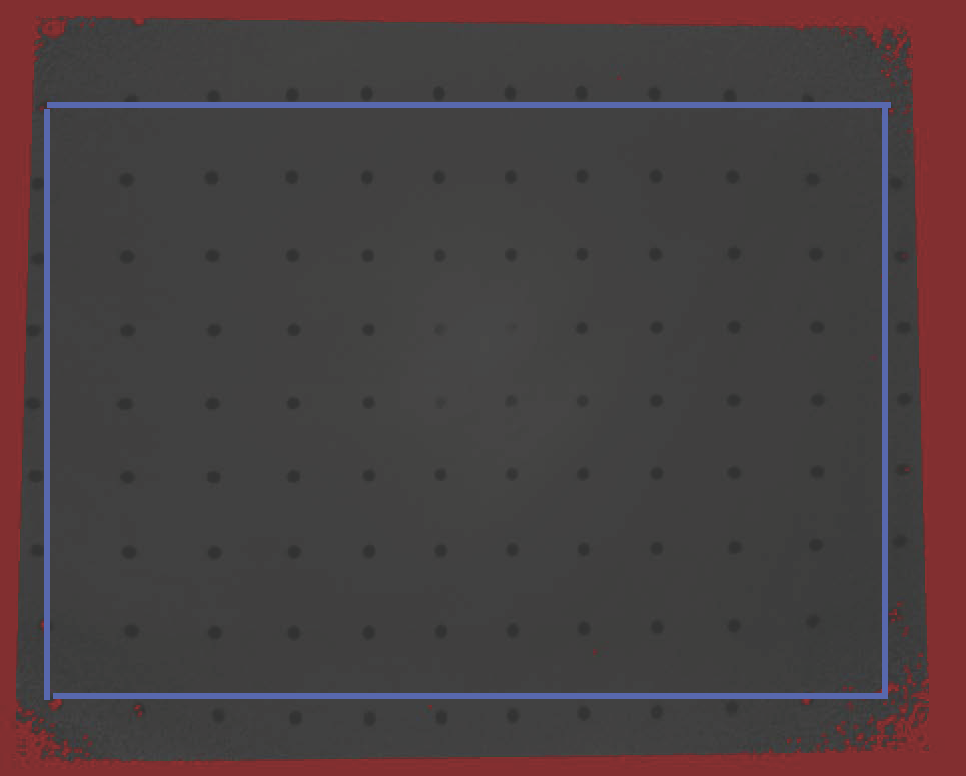
\includegraphics[height=0.42\textwidth]{NIR_by_Depth_front}
%\label{NIR_by_Depth_front}}
%\subfloat[Left View][Left View]{
%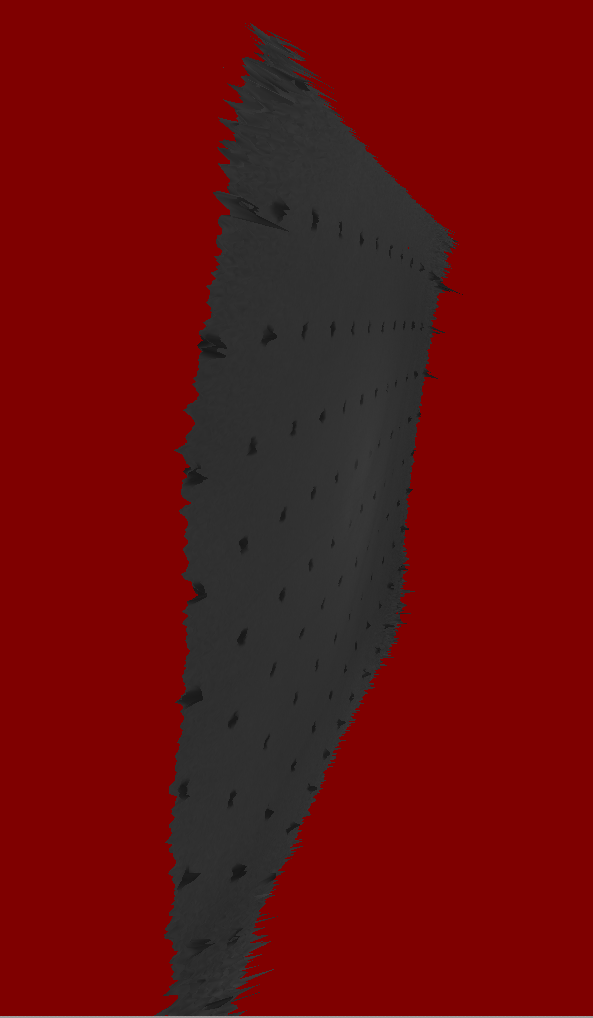
\includegraphics[height=0.42\textwidth , width = 0.4\textwidth]{NIR_by_Depth_LeftSide}
%\label{NIR_by_Depth_LeftSide}}
%%\qquad
%\caption{Raw Distorted KinectV2 NearIR 3D Reconstruction}
%\label{NearIR}
%\end{figure}%
%%
%However, those camera calibration methods, using limited number of points to train the non-linear distortion-removal model, are not able to cover all pixels of a sensor. Besides, with one pinhole camera model (3-by-4 transformation matrix) for raw (deformed) 3D reconstruction and another model to remove lens distortion, the final 3D reconstruction cannot be displayed efficiently in real-time. What's worse, those calibration methods are assuming that the depth sensor offers perfectly same precision depth value for all pixels. Whereas in practical depth sensors always have some defects in getting same depth accuracy for all of their pixels, which we will call as \enquote{Depth Distortion}. Kourosh and Sander \cite{KinectAccuracy_2012} provide an analysis of the accuracy and resolution of Kinect's depth data. They show that the random error of depth measurement increases with increasing distance to the sensor, and ranges from a few millimeters up to about 4 cm at the maximum range of the sensor. Figure~\ref{NIR_by_Depth_LeftSide} shows the side view of KinectV2's raw 3D NearIR image observing the wall, and the blue straight line is added on the left side of the 3D reconstruction. We can tell that most pixels on the left side border are apparently not sitting on a straight line.%
%\\\indent
%%
%\begin{figure}[t]
%\centering
%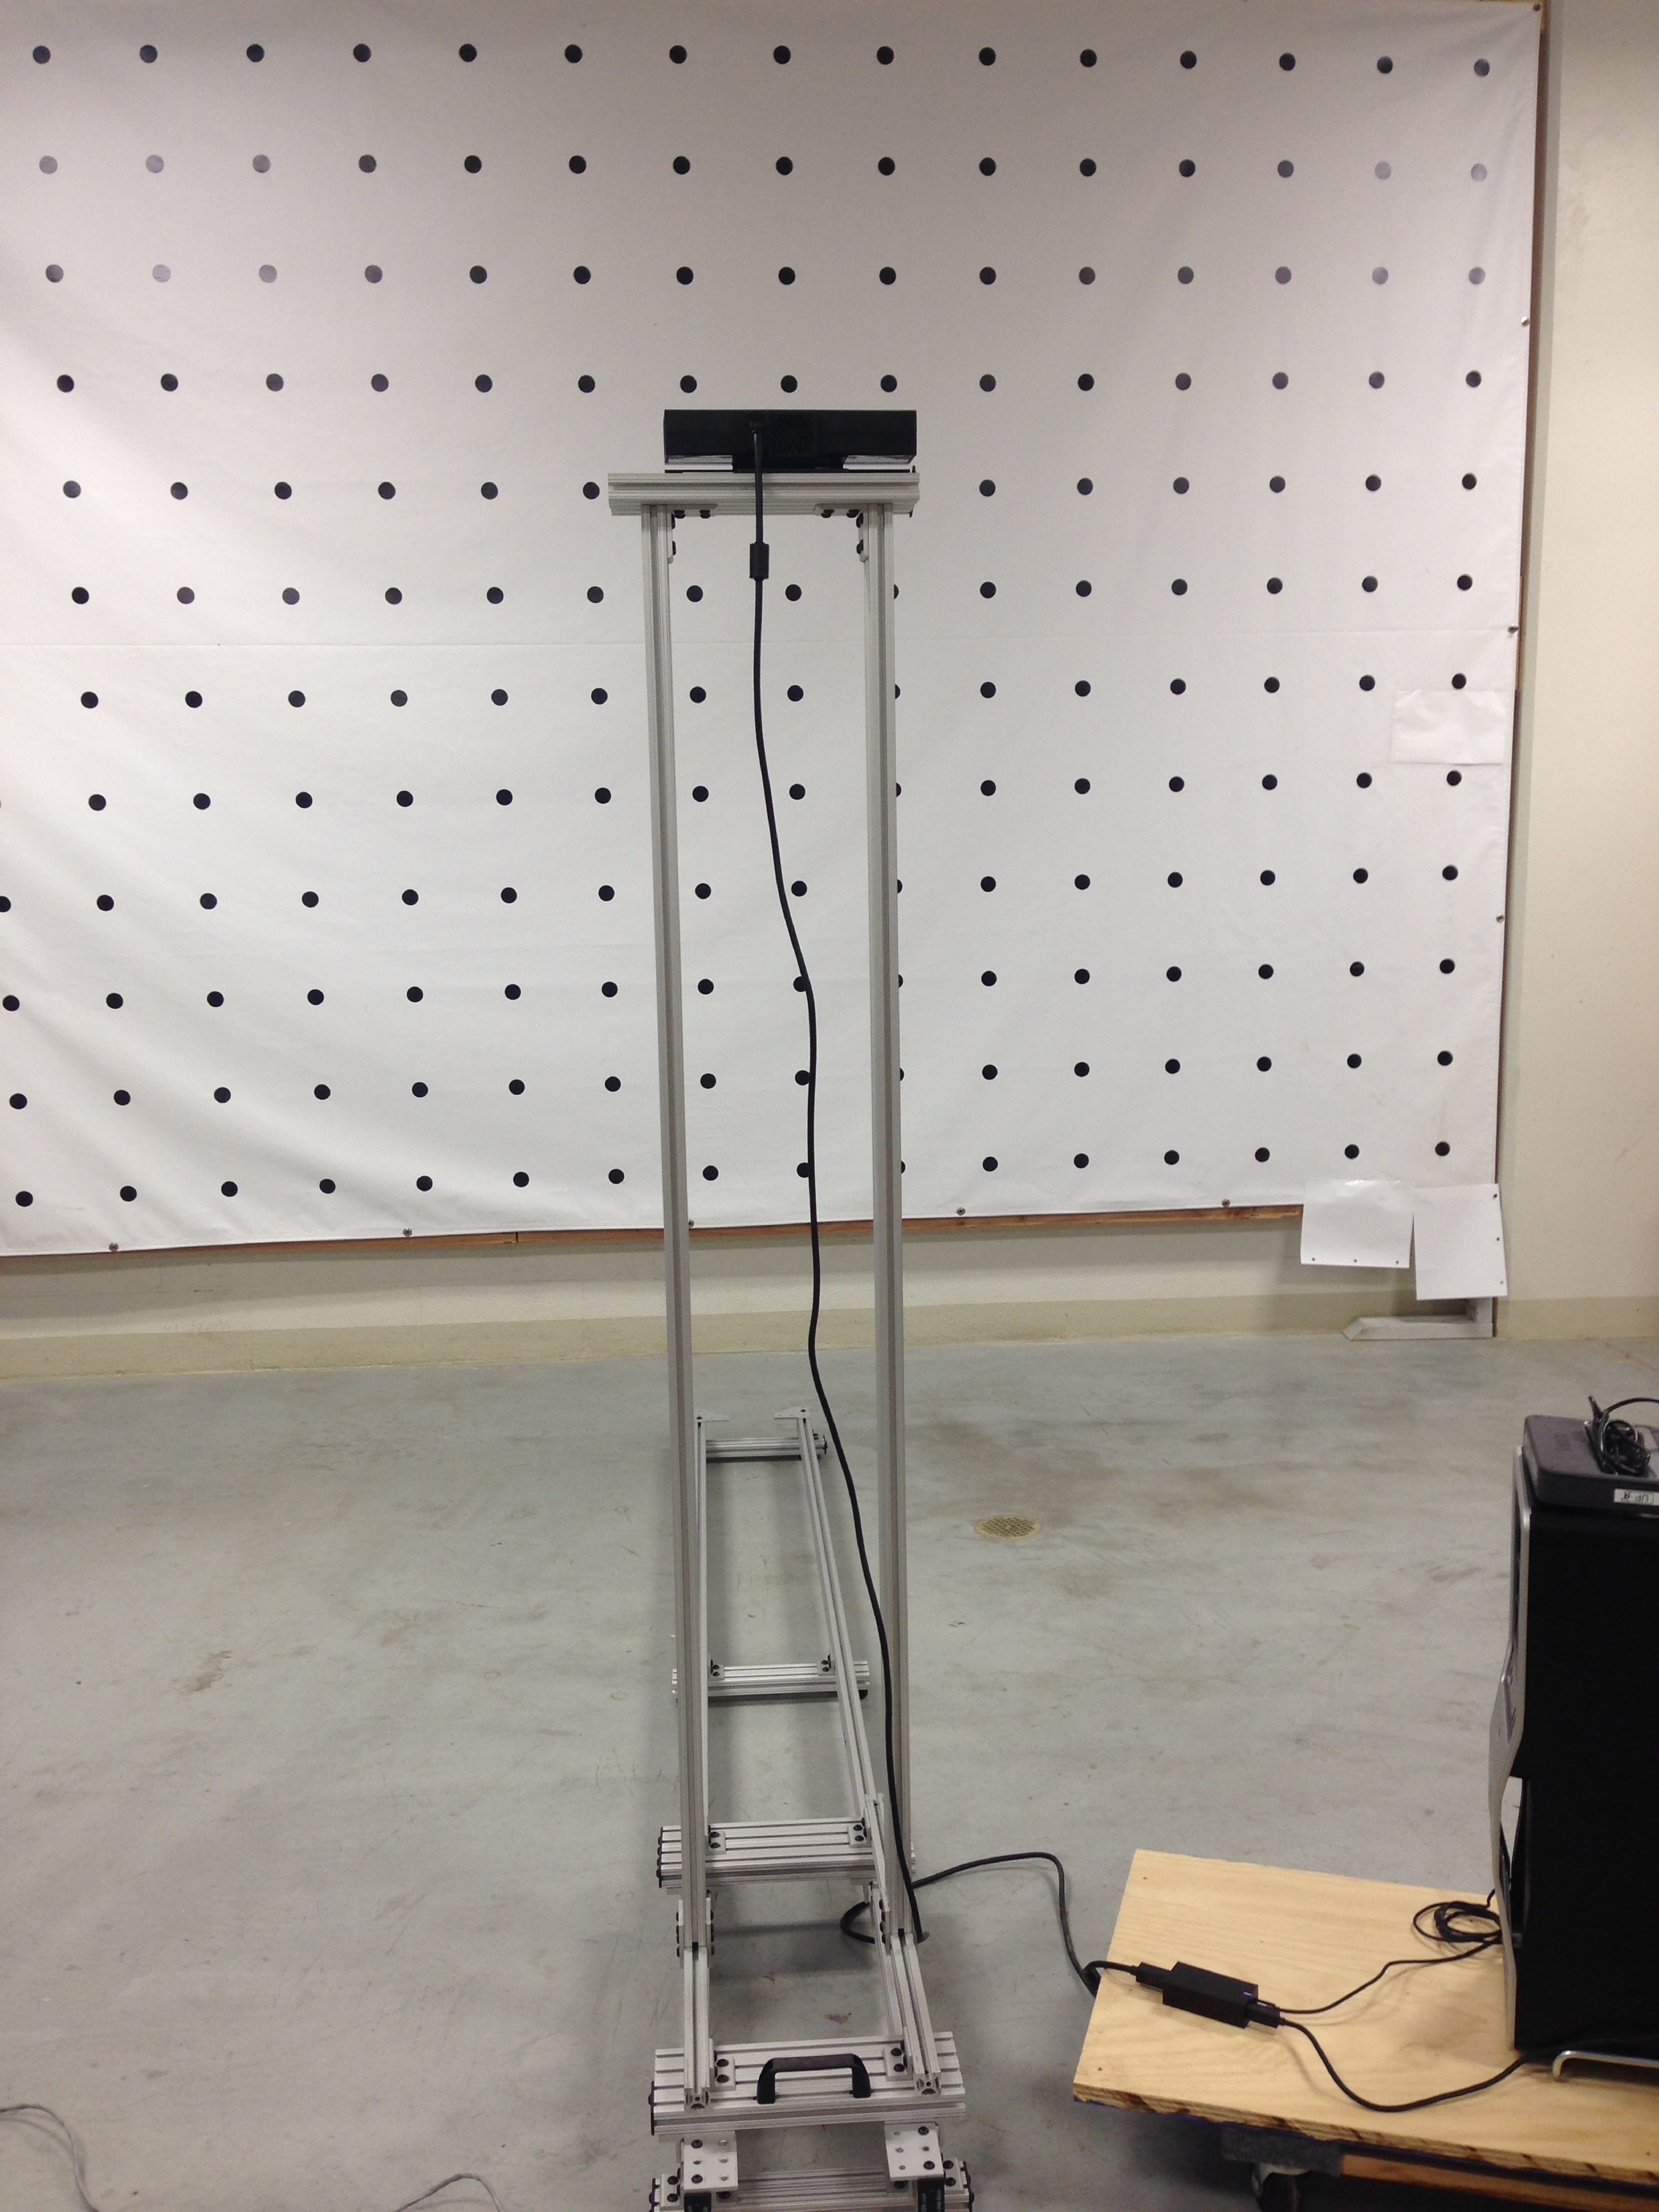
\includegraphics[width=0.55\textwidth]{trackingModuleOnKinectV2CalibrationSystem}
%\caption{KinectV2 Calibration System}
%\label{trackingModuleOnKinectV2CalibrationSystem}
%\end{figure}%
%%
%In order to get enough calibrating points that can cover all pixels of the sensor, as well as solving the \enquote{Depth Distortion}, a moving plane with camera on rail calibration system is introduced in this thesis. As shown in figure \ref{trackingModuleOnKinectV2CalibrationSystem}, the rail is perpendicular to the uniform round dots pattern, along with the \(Z^{w}\) axis. A RGB-D camera KinectV2 is mounted on the top of the slider, whose moving along the rail generates same effect as a moving pattern plane. This calibration system makes it possible to do per-pixel \enquote{Depth Distortion} calibration.%
%%
%
%
%










